\section{Sensor Model, Problem, Related Work}
\label{sec:quantum_problem}

In this section, we describe our mathematical model of a quantum sensor and formulate the quantum transmitter localization problem.
We also briefly talk about related work.

\begin{figure}[h]
    \centering
    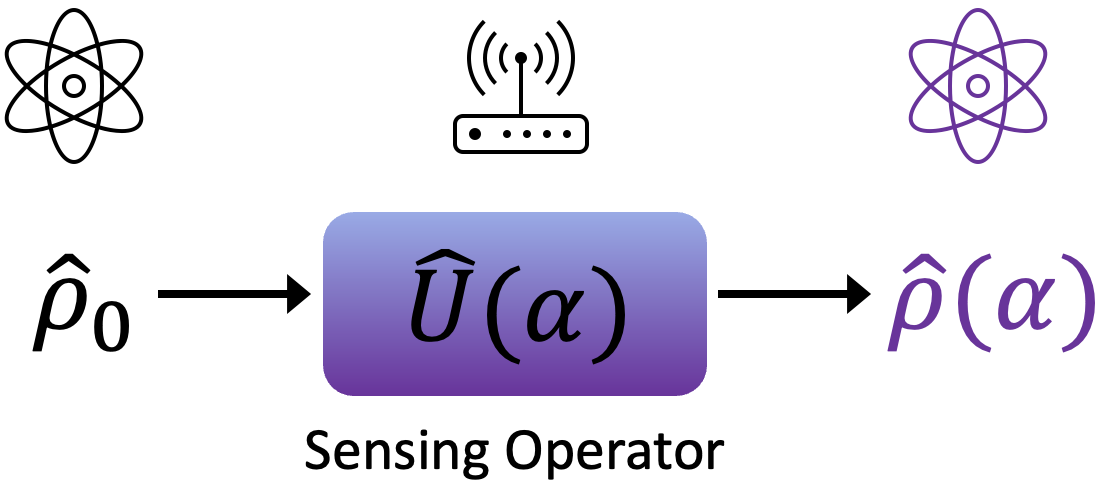
\includegraphics[width=0.5\textwidth]{chapters/qce/figures/unitary.png}
    % \vspace{-0.1in}
    \caption{Sensing modeled as a single parameter estimation problem. The initial state $\hat{\rho}_{0}$ is used to probe an unknown parameter $\alpha$ embedded in the unitary operator $\hat{U}(\alpha)$, yielding output state $\hat{\rho}(\alpha)$.}
    % \vspace{-0.1in}
    \label{fig:unitary}
\end{figure}
\para{The mathematical model of quantum sensors.} We first formulate quantum sensing as a single parameter estimation problem, shown in Fig.~\ref{fig:unitary}.
Consider a parameter $\alpha$ embedded in a unitary operator.
To sense $\alpha$, one prepares an initial quantum state $\hat{\rho}_{0}$ and passes it through unitary operator $\hat{U}(\alpha)$, obtaining the output state:
$\hat{\rho}(\alpha) = \hat{U}(\alpha) \hat{\rho}_{0} \hat{U}^{\dagger}(\alpha)$.
$\hat{U}(\alpha)$ describes the interaction between a qubit and the environment~\cite{arizona21-thesis}
\begin{equation}
    \hat{U}(\alpha) = e^{-i\alpha \hat{G}}
    \label{equ:unitary_generator}
\end{equation}
where $\hat{G}$ is called the generator, which is a Hermitian operator.
$\hat{G}$ is determined by the type of $\alpha$.
The type includes quadrature displacement~\cite{PRL20-qsn}, phase shift~\cite{nature21_phase} and qubit phase rotation, etc,~\cite{Zhang_2021}. 
In this chapter, we assume $\alpha$ is the \emph{phase shift}, and our generator follows the expression in~\cite{nature21_phase}
\begin{equation}
    \hat{G} = \sigma_z / 2 = 
    \begin{bmatrix}
    \frac{1}{2} & 0\\
    0 & -\frac{1}{2}
    \end{bmatrix}
    \label{equ:generator}
\end{equation}
We further assume that the phase shift $\alpha$ is a function of the distance between the transmitter and the sensor.
This assumption is based on the observation that the closer the sensor is to the transmitter, the more affected the sensor is by the transmitter.
If we can build a connection between the transmitter-receiver distance and some properties of the RF wave, we can model the $\hat{U}(\alpha)$ as a function of the RF wave.
In this chapter, we pick received signal strength (RSS) as the bridge that connects the $\alpha$ and the RF wave, because RSS is easily accessible and is widely used in the fingerprinting-based wireless localization field.
We have
\begin{equation}
    \alpha = \frac{2\pi (RSS - NF)}{MP-NF}
    \label{equ:alpha}
\end{equation}
where $NF$ is the noise floor, $MP$ is the maximum power a sensor can receive. 
We have $\alpha \in [0, 2\pi]$, since the received signal strength $RSS \in [NF, MP]$.
Derived from Equation~\ref{equ:unitary_generator}, \ref{equ:generator}, \ref{equ:alpha}, the unitary operator at the sensor can be described as
\begin{equation}
    \hat{U}(\alpha)   = 
    \begin{bmatrix}
    e^{- i \frac{\pi (RSS - NF)}{MP-NF}} & 0\\
    0 & e^{ i \frac{\pi (RSS - NF)}{MP-NF}}
    \end{bmatrix}
    \label{equ:unitary}
\end{equation}
The Equation~\ref{equ:unitary} is interpreted as follows: A quantum sensor is affected by the signal sent by a transmitter.
The transmitter's signal triggers a phase shift in the quantum sensor and a certain value of phase shift is a function of RSS. 
For the RSS model, we use the log-distance model
\begin{equation}
    RSS(d) = P_0 - 10\beta log_{10}(d) + \mathcal{X}
    \label{equ:propagation}
\end{equation}
where $P_0$ is the reference power a sensor receives at 1 meter away from the transmitter, $d$ is the transmitter-receiver distance, $\beta$ is the path-loss exponent, and $\mathcal{X}$ is the shadowing effect that can be represented by a zero-mean Gaussian distribution.

After modeling a single sensor, let us model multiple sensors in a distributed sensing scenario~\cite{Zhang_2021}.
We assume $N$ unknown parameters at $N$ quantum sensors respectively. 
The combined unitary operator is a \emph{tensor product} of $N$ individual unitary operators,
$\hat{U}(\boldsymbol{\alpha}) = \bigotimes_{n=1}^{N} \hat{U}(\alpha_n)$.
To carry out sensing, one inputs $N$ probes in a quantum state $\hat{\boldsymbol{\rho_0}}$ and obtains the output quantum state,
$\hat{\boldsymbol{\rho}}_N({\boldsymbol{\alpha}}) = \hat{U}(\boldsymbol{\alpha}) \hat{\boldsymbol{\rho}_0} \hat{U}^{\dagger}(\boldsymbol{\alpha})$,
where the unknown parameters are $\boldsymbol{\alpha}=\{\alpha_n\}_{n=1}^{N}$, and each $\alpha_n$ represents an unknown parameter at the $n$th sensor. 


\para{Problem Setting and Formal Definition.}
Consider a network of quantum sensors distributed in a geographic area and a single transmitter active in the area.
We assume each quantum sensor holds one qubit. 
For simplicity, we assume all qubits are in pure states, i.e., $\hat{\rho_0} = \ket{\psi_0} \bra{\psi_0}$ and $\ket{\psi_{\alpha}} = \hat{U}(\alpha) \ket{\psi_0}$.
Assume the initial state of the quantum sensor network is 
$\ket{\boldsymbol{\psi_{0}}}$. 
After the interaction with the environment, the quantum state evolves to $\ket{\boldsymbol{\psi_{\alpha}}} = \hat{U}(\boldsymbol{\alpha}) \ket{\boldsymbol{\psi_{0}}}$.
Our problem is to determine the location of the transmitter, given the quantum state $\ket{\boldsymbol{\psi_{\alpha}}}$ reported by the quantum sensor network.


\para{Related Work.}
RF localization has been an active area of research for three decades.
One of the pioneering works is RADAR~\cite{infocom00-radar}.
RADAR is a fingerprinting-based method that has two phases.
In the training phase, a person holds a receiver and travels in an area, meanwhile RADAR records information about the radio signal as a function of the location, i.e., constructs a received signal strength (RSS) fingerprinting map.
In the localization phase, RADAR conducts the nearest neighbor search and reports the location of the closest signal on the fingerprinting map.
The premise is that RSS information provides a means of inferring RF location.
Horus~\cite{mobisys05-horus} improves the localization accuracy by using a probabilistic method.
\eat{and LiFS~\cite{mobicom12-lifs} aims to remove the burden of the site survey process.}
The target to be localized can either be a transmitter~\cite{tx-localization}, a sensor~\cite{infocom00-radar}, or neither both (device-free localization~\cite{devicefree-loc}).
In this work, the target we localize is a single transmitter.
For the simultaneous localization of multiple transmitters, see~\cite{pmc22-deepmtlpro}.

All the localization works above are classical, i.e., they use classical wireless sensors and classical localization methods.
The first localization work that brings in quantum is~\cite{lcn22-qloc}.
It uses quantum amplitude encoding~\cite{slqc} that embeds an RSS vector of length $2^N$ into the amplitudes of an $N$ qubit quantum state. 
Thus, in theory, it brings exponential enhancement in space complexity.
Then, it uses a quantum fingerprinting method based on the quantum cosine similarity algorithm~\cite{PhysRevLett.quantumfingerprint} to match a signal to be localized to a signal recorded in the fingerprinting map.
The work leverages quantum computing and the power of quantum superposition, but they still use classical wireless sensors that collect classical data.



% In this chapter, the quantum sensor is derived from the RF-photonic sensors from~\cite{PRL20-qsn}.
% But our quantum sensors do not do a homodyne measurement.
% Instead, the quantum state at a quantum sensor is teleported to a central node and a global measurement is performed at the central node.
